\documentclass[]{article}
 
\begin{document}
\section{Beschrijving van het project}
\label{Beschrijving}
\subsection{Einddoel van applicatie}
Het einddoel van de applicatie is een visuele IDE met een professioneel uiterlijk en eenvoudige werking. Hierin kunnen event-based programma´s op een intu\"itieve en eenvoudige manier uitgewerkt worden. De uitvoering van blokken kan visueel gevolgd en onderbroken worden in de debug modus. Het doorgeven van Events tussen Instanties kan via wires in het Frame-view. Een visueel canvas kan gebruikt worden om instanties en veranderingen ervan te tonen. Ook kunnen hierin input Events worden gegenereerd op instanties.
\subsection{Interpretatie van opgave}
\label{interpretatie}
Onze interpretatie zorgt ervoor dat de gebruiker op verschillende niveau's programma's kan maken in de IDE. Eenderzijds kan de gebruiker de flow van het programma opbouwen door middel van blokken met elkaar te verbinden. Deze verbindingen worden Events genoemd die uitgelegd staan in Sectie \ref{Events}. Deze flow wordt gemaakt door grote blokken van een bepaald type die bv. een telefoon of drukknop voorstellen, met elkaar te verbinden, dit noemen we Instanties van een type. Door deze flow te maken kan de gebruiker op intu\"{i}tieve wijze een programma opbouwen. Deze flow toont aan wat er gebeurt en wanneer iets gebeurt. \\\\
Anderzijds kan de gebruiker de types van de grote blokken (zie Sectie \ref{Klassen}) opbouwen, dit noemen we een Klasse. Dit gebeurt door een programma te maken van een opeenvolging van kleine blokken. Deze kleine blokken stellen algemene programmeer structuren voor zoals een while-loop. Door deze opbouw kan de gebruiker zien hoe iets werkt. \\\\
Uiteindelijk kan de gebruiker het gemaakte programma runnen. Hierbij kan de gebruiker input events (met behylp van toetsaanslagen en de muis) sturen naar de grote blokken. \\\\ Door het opdelen van het programma naar een niveau waar de gebruiker het wat en wanneer maakt van een programma en een niveau waar hij de hoe maakt, is de IDE laagdrempelig en eenvoudig in gebruik. Er is een console ge\"{i}mplementeerd. In deze console kan de gebruiker ook tekst afprinten. Hierdoor heeft de gebruiker een visueel canvas en de console waar tekst afgeprint in kan worden. Deze console toont ook systeem output, zoals runtime errors.\\\\ 
Dit is ons eindverslag. Eerst wordt er een algemeen beeld gegeven over de IDE waaronder de functionaliteit. Hierna wordt het ontwerp, de gebruikte algoritmes en datastructuren, bekeken. Uiteindelijk geven we mogelijke uitbreidingen voor de IDE aan. In de bijlagen vind u de ge\"{i}mplementeerde kleine blokken, een handleiding, reflectie en een logboek. Ten opzichte van het analyseverslag zijn er verschillende toevoegingen gebeurt. In het analyseverslag was de GUI, en de drag-and-drop niet uitgewerkt. De verdere analyse is hetzelfde gebleven. De algoritmes en datastructuren die bij de analyse gemaakt zijn, bleken goed en effici\"ent te werken.

\subsection{Noden van de opdrachtgever}
\label{Noden}
Naast de algemene features van de applicatie wenst de opdrachtgever dat er aandacht wordt besteed aan volgende punten. Deze staan gerangschikt van meest prioritair naar minder prioritair.
\begin{enumerate}
\item De opdrachtgever wenst een professioneel uiterlijk.
\item De applicatie moet beschikbaar zijn in verschillende talen.
\item De IDE moet bruikbaar zijn door een persoon met beperkte programmeer kennis.
\item De opdrachtgever wenst dat er een debug modus aanwezig is waarin het programma vertraagd wordt afgespeeld en de flow van het programma duidelijk wordt aan de gebruiker.
\item Een door de gebruiker gecree\"{e}rd programma moet opgeslaan worden in een opslag formaat  dat nog leesbaar is in tekstformaat.
\item De opdrachtgever wenst dat er geen globale variabelen aanwezig kunnen zijn in het programma.
\end{enumerate}
 
\subsection{Bestaande Software}
In de volgende sectie worden enkele bestaande software producten besproken. Er wordt uitgelegd welke elementen we overgenomen hebben en welke elementen niet overgenomen zijn.
\label{software}
\subsubsection{Sratch}
Scratch \cite{scratch} is een visuele porgrammeer IDE gemaakt door MIT. Scratch focused meer op kinderen en beschikt daardoor ook over minder complexe programmeer structuren.
\paragraph{ voorstellen van een Sprite.}
Een sprite komt in onze applicatie overeen met een instantie van een Klasse. In onze applicatie heeft een Klasse ook een visuele voorstelling en kan deze ook meerdere uiterlijken hebben. Ook kan een Sprite tekstballonen tonen in het canvas, dit is niet de prioriteit in onze applicatie en dus niet ge\"implementeerd. Het plaatsen en dupliceren van een sprite zal bij ons vervangen door het toevoegen van een of meer Instanties van een reeds bestaande Klasse.
\paragraph{Achtergrond van het canvas.}
Scratch geeft de mogelijkheid om de achtergrond van de canvas ook te behandelen als een sprite. Deze feature is niet van belang voor onze omgeving aangezien we focussen op het event-driven programmeren.
\paragraph{Programmeer Blokken in een Sprite.}
Scratch biedt een hoop mogelijkheden aan om acties te doen met een Sprite. Uit de motion-blokken hebben we enkel de mogelijkheid om de $x$- en $y$-positie van een instantie van een Klasse te veranderen. Uit looks hebben we de mogelijkheid overgenomen om het uiterlijk te veranderen in een eerder ingevoegde appearance. Uit de sound en pen blokken hebben we niets overgenomen.\\\\ Er is de mogelijkheid om een variable te cree\"{e}ren in een Klasse, dit wordt gezien als een private member variabele van die Klasse. \\\\ Uit events hebben we de broadcastblok overgenomen. In onze applicatie heeft het echter de betekenis dat een instantie van de Klasse een uitgaande poort heeft voor dat specifieke event en niet alle instanties van Klassen die op dat event geabboneert zijn het event ontvangen. Ook het abboneren op een event gebeurt bij ons anders zoals besproken in Sectie \ref{Events} Events.\\\\ Uit de control blokken: we hebben de standaard controle structuren zoals een while, if-else, forever.
\\\\Sensing blokken zoals het checken op collision hebben we niet overgenomen.
\\\\ Uit de operators nemen we alle functionaliteit over: logica, String, random en rekenkundige operaties.
\\\\ Uit de categorie More blocks van defines nemen we de functionaliteit over, echter wordt dit voorgesteld bij ons door interne functies. Hierdoor is het ook makkelijker om de flow van het programma in een Klasse te volgen. Bij Scratch is dit onoverzichtelijk en dit willen we vermijden.\\\\
Tenslotte hebben we de blokken een professionelere look dan de blokken van Scratch gegeven. Dit gebeurt door gebruik te maken van strakkere lijnen en neutrale kleuren.
 
\subsubsection{Blockly}
Blockly \cite{blockly} is een visuele programmeer IDE gemaakt door Google. Blockly defini\"{e}ert een imperatieve programmeertaal en is niet event-based zoals onze programmeer IDE. De gemaakte code kan geconverteerd worden naar een gekozen formaat. Dit kan oa. Javascript of Python zijn. \\\\
De blokken zijn gemodelleerd naar puzzelstukjes. Dit maakt het gemakkelijk om te zien hoe de blokken in elkaar gestoken kunnen worden. Blockly is gericht op nieuwe programmeurs. Het versimpelt verschillende programmeerconcepten. Er zijn enkel globale variabelen en lijsten zijn niet nul-based maar \'{e}\'{e}n-based. Variabelen zijn niet case-sensitive en kunnen bestaan uit allerhande tekens (inclusief spaties).
\begin{figure}[H]
\centering
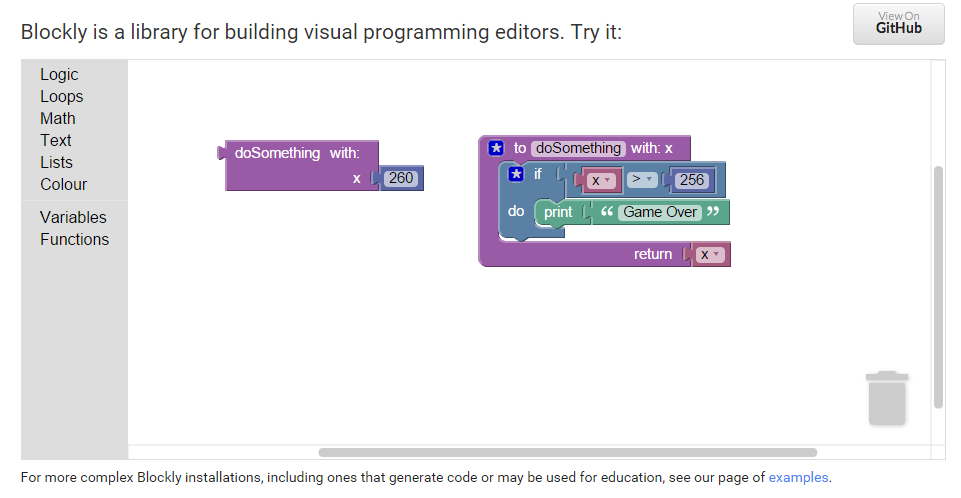
\includegraphics[width=1.2\textwidth]{./BestaandeSoftware/blockly.PNG}
\caption{Blockly.}
\end{figure}
\paragraph{Functies}
Blocky laat toe om functies te cree\"{e}ren. Functies kunnen parameters meekrijgen. Deze functies zijn globaal en kunnen vervolgens op elke plaats in het programma opgeroepen worden. Deze functies zijn gelijkaardig aan de functies van ons project. Echter behoren onze functies tot een bepaalde Klasse.
\paragraph{Operator Blokken}
Ons concept om operatoren toe te passen is gelijkaardig aan het concept dat Blockly gebruikt. Er is slechts 1 operator blok voor de binaire arithmische operatoren, alsook \'{e}\'{e}n operator blok voor de binaire logische vergelijkings operatoren. 
\begin{figure}[H]
\centering
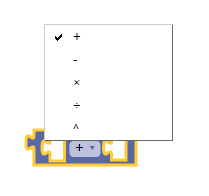
\includegraphics[width=0.4\textwidth]{./BestaandeSoftware/blocklyopp.PNG}
\caption{Blockly operators.}
\end{figure}
\subsubsection{Unreal Engine 4: Blueprints}
De Unreal Engine 4 \cite{unreal} is een game engine die uitgebracht is door Epic Games. In de Unreal Engine 4 is een visueel scripting systeem ingebouwd. Dit wordt Blueprints genoemd. Het laat toe om volledige gameplay elementen visueel te scripten via een node-based interface. Het is mogelijk om een volledige game te implementeren in Blueprints.
\begin{figure}[H]
\centering
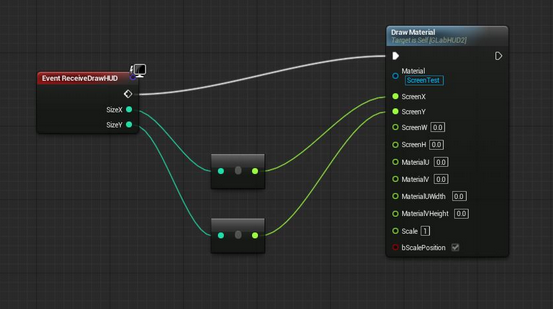
\includegraphics[width=1.1\textwidth]{./BestaandeSoftware/unrealEngine.PNG}
\caption{Unreal Engine 4.}
\end{figure}
De Unreal Engine gebruikt standaard enkel C++ code, ook voor de scripting. Blueprints compilen achterliggend ook naar C++ code. Hierdoor is er geen interpreting nodig van de nodes en is er ook geen snelheidsverlies.
\paragraph{Nodes}
In de Unreal Engine kunnen nodes verbonden worden met elkaar. Dit duidt op een opeenvolging, net zoals er in een imperatief programma de uitvoering van ene instructie overgaat naar de andere. Dit is te zien als de witte lijn. Vervolgens kunnen parameters doorgegeven worden, dit zijn de gekleurde lijnen. Dit kan vergeleken worden met ons systeem in het wireFrame. In ons systeem worden echter events met elkaar doorverbonden en niet de functies. \cite{unreal}
\paragraph{Events}
Het beginpunt van een flow van nodes in de Unreal Engine is een event dat ontvangen word. Dit kan een eigen gemaakt event zijn, of dit kan een standaard events zijn zoals te zien in de afbeelding.
\end{document}